\documentclass[a4paper,12pt]{article}
\usepackage{graphicx}
\usepackage[utf8]{inputenc}
\usepackage[T1]{fontenc}
\usepackage[MeX]{polski}
\usepackage{titling}
\pagestyle{plain}
\title{Dokumentacja projektu Mrówka Langtona}
\author{Mikołaj Kubik 291083, Karol Stasiak 291107}
\date{\today}
\begin{document}
\begin{titlingpage}
\begin{center}
\begin{huge} 
\textbf{\thetitle}\\
\end{huge}
\vspace{0.2cm}
ver. 1.0 \\
\begin{center}
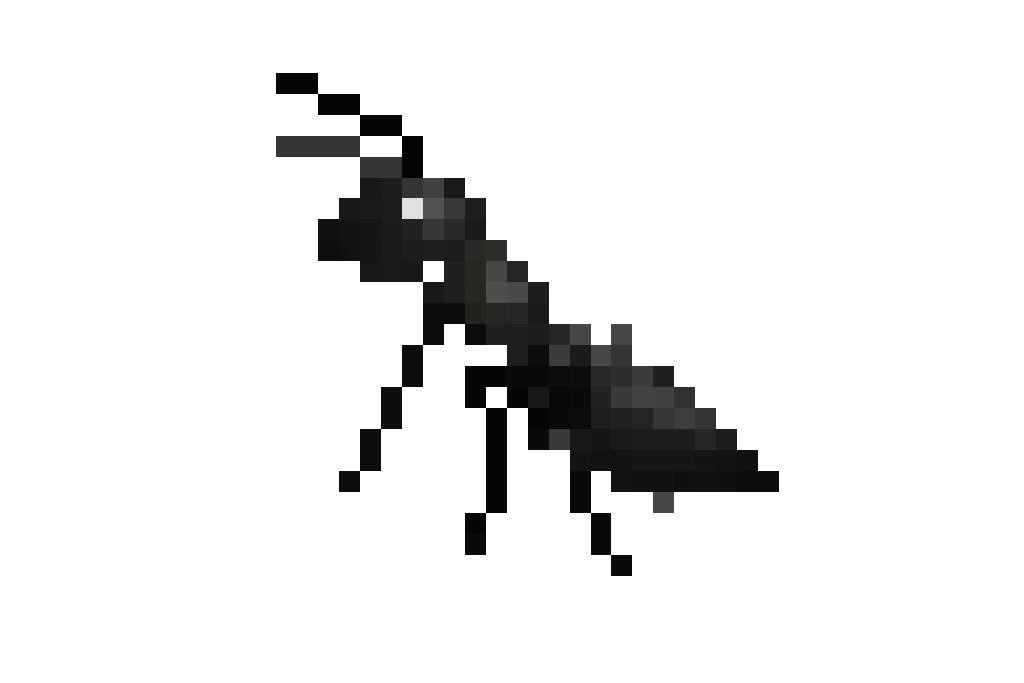
\includegraphics[height=3cm]{logo}
\end{center}
\vspace{0.2cm}
\theauthor\\
\vspace{0.2cm}
Grupa 15\\
\vspace{0.2cm}
\thedate\\
\vspace{0.5cm}
\begin{tabular}{|r|l|l|l|} \hline
wersja & zmiany & kto & kiedy \\
\hline
0.1 & Stworzenie dokumentu & KS & 21.03.2018 \\
\hline
0.2 & Edycja sekcji & MK & 02.04.2018 \\
\hline
0.3 & Edycja sekcji & KS & 03.04.2018 \\
\hline
1.0 & Zatwierdzenie dokumentu & MK & 03.04.2018 \\
\hline
\end{tabular} \\
\vspace{5,2cm}

\includegraphics[height=3cm]{ee}\\
\begin{large}
Politechnika Warszawska\\
Wydział Elektryczny\\
\end{large} 
\end{center}
\end{titlingpage}
\tableofcontents
\newpage
\section{Zasada działania mrówki}
\begin{enumerate}
\item Jeśli znajdzie się na polu białym to obraca się w lewo (o kąt prosty), zmienia kolor pola na swój kolor i przechodzi na następną komórkę;
\item Jeśli znajduje się na polu zakolorowanym to obraca się w prawo (o kąt prosty), zmienia kolor pola na biały i przechodzi na następną komórkę;
\item Porusza się na nieskończonej planszy podzielonej na kwadratowe komórki (zakolorowane lub nie), o rozmiarze 1 px każda;
\item Mrówki startują z wylosowanego miejsca na planszy;
\end{enumerate}
\section{Założenia projektu}
\begin{enumerate}
\item Program obrazuje symulację mrówki Langtona.
\item Program może zostać uruchomiony zarówno z ustawieniami domyślnymi, jak i podanymi przez użytkownika
\item Jeżeli użytkownik poda błędne argumenty, program zadziała zgodnie z argumentami domyślnymi dla danego parametru oraz wyświetli błąd.
\item Program może wyświetlić również animację ruchu mrówek w terminalu.
\item Użytkownik może podać dane zarówno z linii komend, jak i pliku tekstowego.
\item Maksymalne wymiary planszy wynoszą n x m.
\item Program pozwala symulować zachowanie do x mrówek.
\item Mrówki mogą wykonać maksymalnie x kroków.
\item Stan planszy po wykonaniu zadania zostaje zapisany do pliku png.
\item Po dojściu do skraju planszy mrówka automatycznie przechodzi na jej przeciwległy brzeg.
\item Początkowe współrzędne mrówek są ustawiane losowo w przypadku podawania argumentów z linii komend.
\item Początkowe współrzędne mrówek są pobierane z pliku, w przypadku podawania argumentów z pliku tekstowego.
\end{enumerate}
\section{Domyślne ustawienia}
\begin{itemize}
\item \textbf{Wymiary planszy:} 184 x 184
\item \textbf{Liczba mrówek:} 1
\item \textbf{Ilość kroków:} 11000
\item \textbf{Współrzędne początkowe:} Losowe
\end{itemize}
\section{Uruchamianie programu}
Argumenty dla programu (rozmiar planszy oraz liczba mrówek) mogą zostać podane zarówno z terminalu, jak i pliku tekstowego. Zastosowanie podanych wyżej przedrostków x (x to dany przedrostek) pozwoli na wpisywanie danych bez konieczności zachowania odpowiedniej kolejności.
\begin{itemize}
\item Nazwa wywoływanego programu \textbf{./ant}
\item Szerokość planszy \textbf{-w}
\item Wysokość planszy \textbf{-h}
\item Ilość mrówek \textbf{-q}
\item Ilość kroków \textbf{-n}
\item Czy wyświetlić animację w terminalu \textbf{-a}
\item Nazwa pliku w którym ma zostać zapisany obraz \textbf{-o}
\item Nazwa pliku z danymi \textbf{-i}
\end{itemize}
\newpage
\section{Obsługa błędów}
\begin{itemize}
\item Jeżeli wśród argumentów znajdzie się zmienna niebędąca liczbą, program zakończy swoje działanie oraz powiadomi o błędzie.
\item Jeżeli którykolwiek argument przekroczy zakres podany w założeniach, program zatrzyma się i poprosi o poprawę.
\item Jeżeli liczba argumentów będzie zbyt duża, argumenty dodatkowe zostaną zignorowane.
\item Jeżeli użytkownik poda pozycje startowe mrówek wykraczające poza planszę, program zakończy działanie oraz wyświetli informację o błędzie.
\item Jeżeli ilość współrzędnych startowych nie będzie zgadzała się z ilością mrówek, mrówki zostaną rozmieszczone losowo.
\end{itemize}
\section{Budowa programu}
Program podzieliliśmy na 5 części, aby ułatwić czytelność, modyfikacje oraz testy.
\begin{itemize}
\item \textbf{ant.c, ant.h} - odpowiada za implementację struktur ant\_t i ants\_t oraz sposobu poruszania się mrówek 
\begin{itemize}
\item struct* ant\_t
\item struct* ants\_t
\item void move(ant\_t, int)
\item void mirror(ant\_t, int ,int)
\item ants\_t ants\_init(int)
\item void free\_ants(ants\_t)
\end{itemize}
\newpage
\item \textbf{matrix.c, matrix.h} - odpowiada za implementację struktury mat\_t, odpowiednią alokację pamięci na nią oraz opcjonalną animację mrówki w terminalu
\begin{itemize}
\item struct* mat\_t
\item mat\_t init(int, int)
\item void animate(mat\_t)
\item free\_matrix(mat\_t)
\end{itemize}
\item \textbf{exporttopng.c, exporttopng.h} - odpowiada za zapis planszy do pliku png
\begin{itemize}
\item void write\_png\_file(char*)
\item void process\_file(mat\_t)
\end{itemize} 
\item \textbf{error.c, error.h} - odpowiada za obsługę błędów
\begin{itemize}
\item Cuś tu będzie jak zrobimy obsługę
\end{itemize}
\item \textbf{main.c} - odpowiada za sterowanie programem. Działa jako reguła \textbf{main}.
\end{itemize}
Do programu dodatkowo załączyliśmy plik z regułą Makefile, mający na celu uproszczenie kompilacji oraz usuwania plików tymczasowych tworzonych przez program.
\section{Opis poszczególnych modułów}
\subsection{ant.c}
\subsection{matrix.c}
\subsection{exporttopng.c}
\subsection{error.c}
\subsection{main.c}
\newpage
\section{Przykładowe wywołanie}
\textbf{Zastosowane zostały domyślne wartości}
\begin{center}

\includegraphics[height=10cm]{out}
\end{center}
\end{document}